%%
\documentclass[11pt,a4paper,english,greek,twoside]{ceid-thesis}

\usepackage{graphicx}
\usepackage{epstopdf}
\usepackage{indentfirst}
\usepackage{verbatim}
\usepackage{amsmath}
\usepackage{amsthm}
\usepackage{amssymb}
\usepackage{latexsym}
\bibliographystyle{static/hellas}
\usepackage{hyphenat}
\usepackage{makeidx}
\addto\captionsgreek{%
  \renewcommand{\indexname}{Ευρετήριο όρων}%
}
\makeindex

% 1.5 spacing
\renewcommand{\baselinestretch}{1.2}

% latin text (and greek text)
\newcommand{\tl}[1]{\textlatin{#1}}
\newcommand{\tg}[1]{\textgreek{#1}}

% typeset short english phrases
\newcommand{\en}[1]{\foreignlanguage{english}{#1}}

% typeset source code
\newcommand{\src}[1]{{\tt\en{#1}}}

% typeset a backslash
\newcommand{\bkslash}{\en{\symbol{92}}}

\newtheorem{definition}{Ορισμός}
\newtheorem{proposition}{Πρόταση}
\newtheorem{theorem}{Θεώρημα}
\newtheorem{corollary}{Συμπέρασμα}
\newtheorem{lemma}{Λήμμα}
\newtheorem{example}{Παράδειγμα}
\newtheorem{remark}{Σημείωση}
\newtheorem{notation}{Συμβολισμός}
\newtheorem{law}{Νόμος}
\renewcommand{\thedefinition}{\arabic{chapter}.\arabic{definition}}
\renewcommand{\theproposition}{\arabic{chapter}.\arabic{proposition}}
\renewcommand{\thetheorem}{\arabic{chapter}.\arabic{theorem}}
\renewcommand{\thecorollary}{\arabic{chapter}.\arabic{corollary}}
\renewcommand{\thelemma}{\arabic{chapter}.\arabic{lemma}}
\renewcommand{\theexample}{\arabic{chapter}.\arabic{example}}
\newcommand{\set}[1]{\left\{#1\right\}}
\newcommand{\To}{\Longrightarrow}
\newcommand{\xml}{\en{XML}}

\selectlanguage{greek}

\hyphenation{ο-ποί-α}

%%%%%%%%%%%%%%%%%%%%%%%%%%%%%%%%%%%%%%%%%%%%%%%%%%%%%
%% THESIS INFO 
%%
%
% Τίτλος Πτυχιακής Εργασίας
	\title{Αναζήτηση και Εξόρυξη Πληροφορίας σε Μεγάλες Βάσεις Αδόμητων Δεδομένων με Μεθόδους Παράλληλης Επεξεργασία}
% "του" ή "της", ανάλογα με το φύλο του σπουδαστή
	\edef\toutis{της}
% Ονοματεπώνυμο σπουδαστή (ΚΕΦΑΛΑΙΑ, γενική πτώση)
	\edef\authorNameCapital{ΤΣΑΜΟΥ ΟΛΥΜΠΙΑΣ}
% Ονοματεπώνυμο σπουδαστή (πεζά, ονομαστική πτώση)
	\author{Ολυμπία Τσάμου}
% Ονοματεπώνυμο Επιβλέποντα Καθηγητή
	\supervisor{Ευάγγελος Δερματάς}
    \edef\supervisorTitle{Καθηγητής}
% Ονοματεπώνυμο Επιβλέποντα Καθηγητή
	\supervisorSecond{}
    \edef\supervisorSecondTitle{**** Τίτλος}
% "Επιβλέπων" ή "Επιβλέπουσα", ανάλογα με το φύλο του Επιβλέποντα Καθηγητή
	\edef\supervisorMaleFemale{Επιβλέποντες}
% Τόπος, μήνας και έτος
	\edef\thesisPlaceDate{Πάτρα, Μάιος 2022}
% Ημερομηνία Εξέτασης
	\edef\examinationDate{19η Μαΐου 2022}
% Έτος Copyright
	\edef\copyrightYear{2022}
% Ονοματεπώνυμο 1ου εξεταστή
	\epitropiF{Θεόδωρος Αντωνακόπουλος}
% Τίτλος 1ου εξεταστή
	\edef\epitropiFTitle{Καθηγητής}
% Ονοματεπώνυμο 2ου εξεταστή
	\epitropiS{****}
% τίτλος 2ου εξεταστή
	\edef\epitropiSTitle{Καθηγητής}
%%%%%%%%%%%%%%%%%%%%%%%%%%%%%%%%%%%%%%%%%%%%%%%%%%%%%


\begin{document}
\selectlanguage{greek}
\maketitle

\frontmatter
% Περίληψη
	\begin{abstract}
Περίληψη


   \begin{keywords}
   Παράλληλος Προγραμματισμός, Συνελικτικά Νευρωνικά Δίκτυα, \tl{OpenACC}, Αναγνώριση Εικόνας
   \end{keywords}
\end{abstract}



\begin{abstracteng}
\tl{Abstract}

   \begin{keywordseng}
    \tl{Parallel Programming, Convolutional Neural Networks, OpenACC,Image Classification}
   \end{keywordseng}

\end{abstracteng}
% Αφιέρωση
	\thesisDedication{στους γονείς μου}
% Ευχαριστίες
	\begin{acknowledgements}
Θα ήθελα καταρχήν να ευχαριστήσω τον καθηγητή κ. .........
για την επίβλεψη αυτής της διπλωματικής εργασίας [ ] ευχαριστώ ιδιαίτερα τον Δρ.
............ για την καθοδήγησή του και την εξαιρετική
συνεργασία που είχαμε. Τέλος θα ήθελα να ευχαριστήσω τους γονείς
μου για την καθοδήγηση και την ηθική συμπαράσταση που μου
προσέφεραν όλα αυτά τα χρόνια.
\end{acknowledgements}
% Πίνακας Περιεχομένων
	\tableofcontents
% Κατάλογος Σχημάτων
	\listoffigures
% Κατάλογος Πινάκων
	\listoftables

%%%%%%%%%%%%%%%%%%%%%%%%%%%%%%%%%%%%%%%%%%%%%%%%%%%%%
%% INCLUDE YOUR CHAPTERS/SECTIONS HERE
%%
\mainmatter
% Εισαγωγή
	\chapter{Εισαγωγή}

Εισαγωγή.\cite{zoi04}

\section{Ορισμός του Προβλήματος}
Εφαρμογή τεχνικών βελτιστοποίησης σε πρόβλημα ταξινόμησης εικόνων κάνοντας χρήση ενός Συνελικτικού Νευρωνικού Δικτύου \cite{cs61c}


\section{Στόχοι της Διπλωματικής Εργασίας}

Γίνεται έρευνα σχετικά με τις διαφορετικές αρχιτεκτονικές νευρωνικών δικτύων και τις μεθόδους εκπαίδευσης, ωστόσο, μια άλλη κρίσιμη πτυχή των νευρωνικών δικτύων είναι, δεδομένου ενός εκπαιδευμένου δικτύου, η γρήγορη και ακριβής ταξινόμηση εικόνων.
Σε αυτό το \en{project}, δίνετε ένα εκπαιδευμένο νευρωνικό δίκτυο που ταξινομεί εικόνες 32\en{x}32 \en{RGB} σε 10 κατηγορίες. Οι εικόνες ανήκουν στο \en{dataset  CIFAR-10}. Μας δίνετε ο αλγόριθμος εμπρόσθιας διάδοσης του νευρωνικού δικτύου και τα τελικά βάρη του δικτύου. Σκοπός είναι η βελτίωση της ταχύτητας της εμπρόσθιας διάδοσης ώστε να γίνει ταξινόμηση με πιο γρήγορο ρυθμό.

% Κεφάλαια
	\chapter{\selectlanguage{greek}Θεωρητικό Υπόβαθρο}
Κατηγοριοποίηση Εικόνων με χρήση Συνελικτικών Νευρωνικών Δικτύων  
\en{classifying images using a Convolutional Neural Network}

\section{Αναγνώριση Εικόνων}
\subsection{Πώς ένας υπολογιστής αναγνωρίζει εικόνες;}
Η ταξινόμηση εικόνων περιγράφει ένα πρόβλημα στο οποίο σε ένα υπολογιστή δίνεται μία εικόνα και πρέπει να καταλάβει τι απεικονίζει (από ένα σύνολο πιθανών κατηγοριών)
Σήμερα, τα Συνελικτικά Νευρωνικά Δίκτυα (\en{CNNs}) αποτελούν  μια πολύ καλή  προσέγγιση αυτού το προβλήματος. Γενικά, τα νευρωνικά δίκτυα υποθέτουν πως υπάρχει κάποια συνάρτηση από την είσοδο (π.χ. εικόνες) σε μία έξοδο (π.χ. ένα σύνολο κατηγοριών εικόνων). Ενώ οι κλασσικοί αλγόριθμοι προσπαθούν να κωδικοποιήσουν  κάποια πληροφορία του πραγματικού κόσμου στη συνάρτηση τους, τα \en{CNN} μαθαίνουν την συνάρτηση δυναμικά  από ένα σύνολο ταξινομημένων εικόνων (\en{labelled images})—αυτή η διαδικασία ονομάζετε εκπαίδευση. Μόλις καταλήξει σε μια σταθερή συνάρτηση (δηλαδή σε μια προσέγγιση αυτής), μπορεί να εφαρμόσει τη συνάρτηση σε εικόνες που δεν έχει ξαναδεί.
\subsection{Τι μπορεί να κάνει ένα νευρωνικό δίκτυο;}
Ένα νευρωνικό δίκτυο αποτελείται από πολλαπλά επίπεδα.  Κάθε επίπεδο λαμβάνει έναν πολυδιάστατο πίνακα αριθμών ως είσοδο και παράγει έναν άλλο πολυδιάστατο πίνακα αριθμών ως έξοδο (ο οποίος στη συνέχεια γίνεται η είσοδος του επόμενου επιπέδου). Κατά την ταξινόμηση εικόνων, η είσοδος του πρώτου επιπέδου είναι η εικόνα εισόδου  (π.χ. 32\en{x}32\en{x}3 αριθμοί για εικόνες 32\en{x}32 \en{pixel} με 3 κανάλια χρώματος), ενώ η έξοδος του τελευταίου επιπέδου αποτελείται  ένα σύνολο πιθανοτήτων των διαφόρων κατηγοριών (π.χ., 1\en{x}1\en{x}10 αριθμοί αν υπάρχουν 10 κατηγορίες).

\begin{figure}[!ht] \centering 
%\includegraphics[width=\textwidth]{universe}
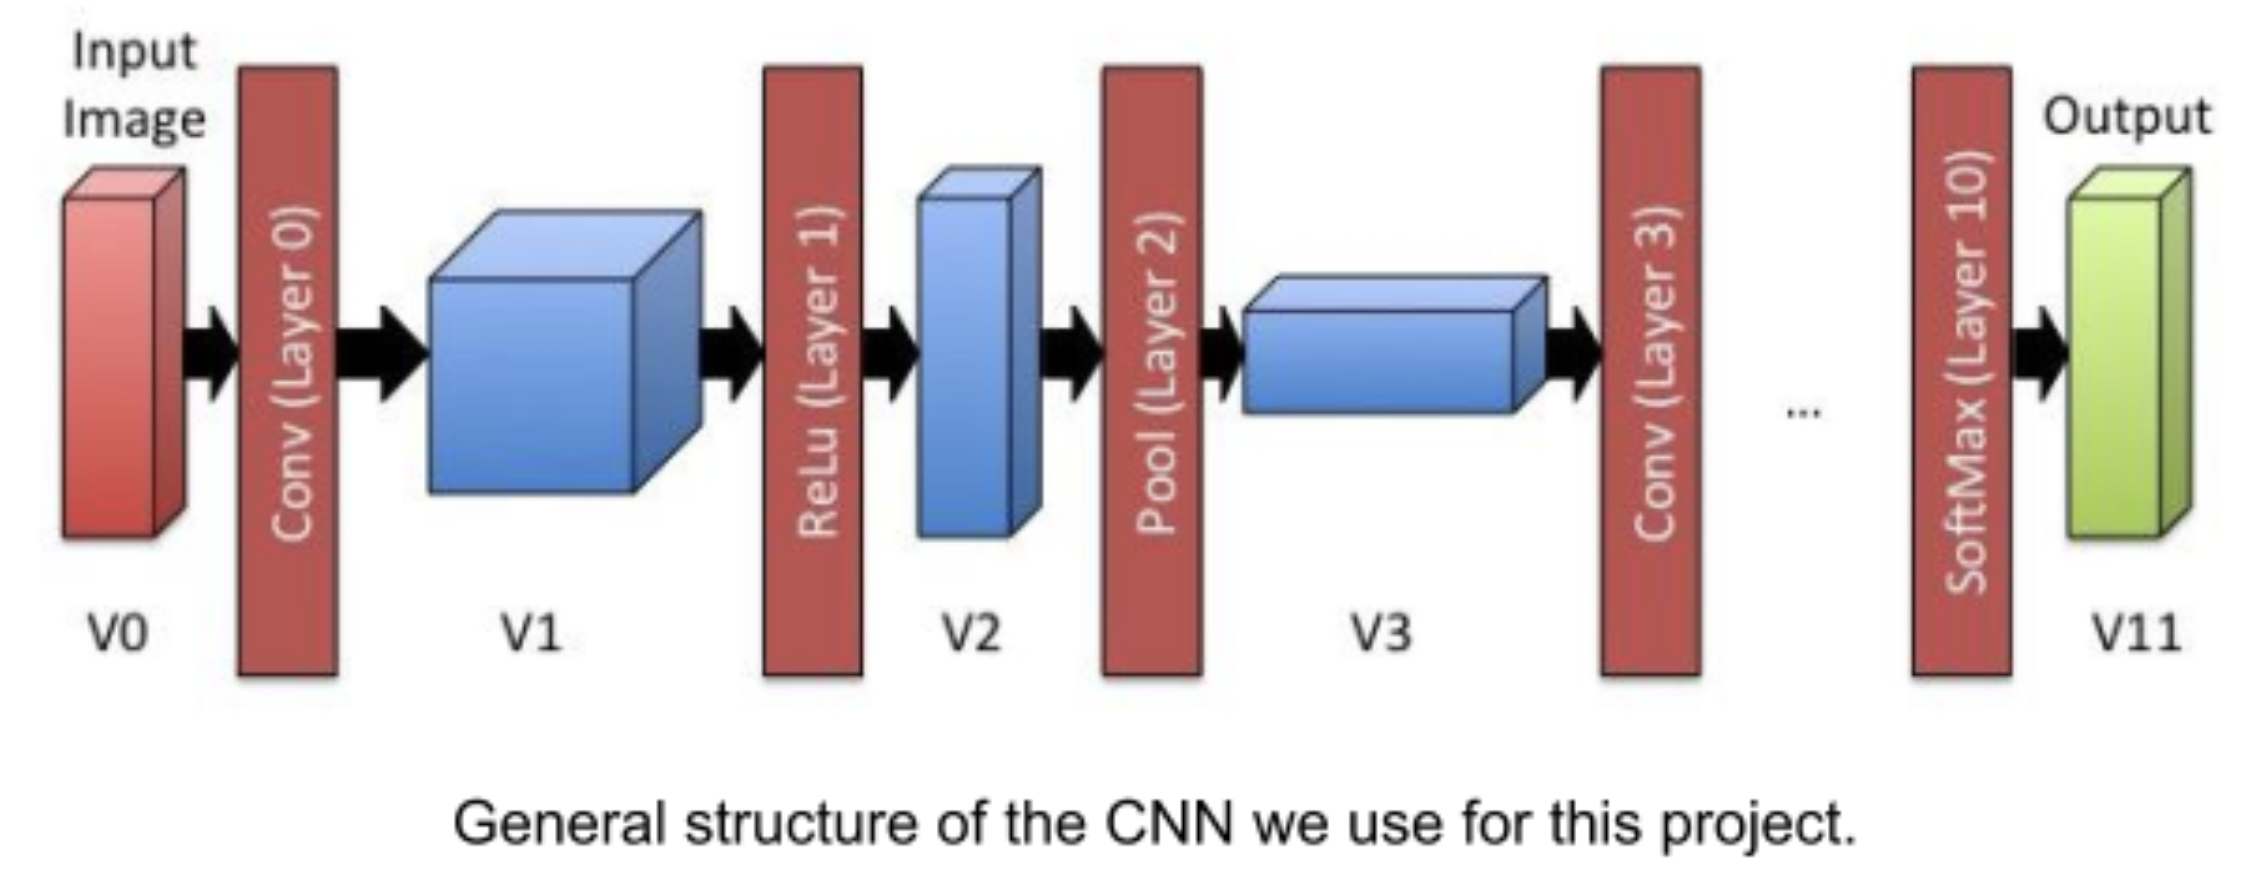
\includegraphics[width=\textwidth]{static/figures/network.png} \caption{Δομή Συνελικτικού Νευρωνικού Δικτύου}\label{figureCNN}
\end{figure}

Αρχιτεκτονική \en{CNN}~\ref{figureCNN} 

Κάθε επίπεδο έχει ένα σύνολο από βάρη που σχετίζονται με αυτό — αυτά τα βάρη είναι που “μαθαίνει” το νευρωνικό όταν του δοθούν δεδομένα εκπαίδευσης. Ανάλογα με το επίπεδο, τα βάρη έχουν διαφορετικές ερμηνείες, αλλά δεν είναι αντικείμενο μελέτης του συγκεκριμένου \en{project}, φτάνει να γνωρίζουμε ότι κάθε επίπεδο λαμβάνει μία είσοδο, εκτελεί κάποια διεργασία σε αυτή, που εξαρτάται από τα βάρη και παράγει μια έξοδο. Αυτό το βήμα ονομάζεται \en{forward pass}: παίρνουμε μία είσοδο και την προωθούμε στο δίκτυο, παράγοντας το επιθυμητό αποτέλεσμα ως έξοδο. Το \en{forward pass} είναι το μόνο που χρειάζεται για την ταξινόμηση εικόνων σε ένα ήδη εκπαιδευμένο \en{CNN}.
    

Στην πράξη, ένα νευρωνικό δίκτυο αποτελεί μια πολύ απλή μηχανή αναγνώρισης προτύπων (με εξαιρετικά περιορισμένη χωρητικότητα), αλλά μπορεί να είναι αρκετά παράξενο αυτό που καταλήγει να αναγνωρίσει. Για παράδειγμα, κάποιος μπορεί να εκπαιδεύσει ένα νευρωνικό δίκτυο να αναγνωρίζει τη διαφορά μεταξύ “σκύλων” και “λύκων”, και να δουλέψει καλά κοιτώντας το χιόνι και το δάσος στο φόντο των φωτογραφιών με τους λύκους.


	\chapter{Περιγραφή θέματος}
Στο κεφάλαιο αυτό αρχικά γίνεται μια περιγραφή των συστημάτων
ομότιμων κόμβων που είναι βασισμένα σε σχήματα \en{(schema-based
peer-to-peer systems)}. Στη συνέχεια περιγράφονται τρία βασικά
συστήματα που ανήκουν σε αυτή την κατηγορία, καθώς και ένα σύστημα
για τη διαχείρηση \en{RDF} σχημάτων, και τέλος αναλύεται ο στόχος
της παρούσας εργασίας.

\section{Σχετικές εργασίες}
Οι βάσεις δεδομένων εισήγαγαν ένα τρόπο αποθήκευσης και ανάκτησης
των δεδομένων που βασιζόταν στο σχήμα \cite{neidl03issues}. Τα
πρώτα συστήματα ομότιμων κόμβων που περιγράψαμε στην Υποενότητα
2.1.2 έδιναν μεγάλη σημασία στην αρχιτεκτονική του συστήματος και
την δρομολόγηση των ερωτήσεων και λιγότερη στον τρόπο
αναπαράστασης και τις δυνατότητες αναζήτησης. Η αναζήτηση σε αυτά
τα συστήματα ομότιμων κόμβων γίνεται με βάση προκαθορισμένα
χαρακτηριστικά - δείκτες, ή με προσπάθεια αντιστοίχισης μιας λέξης
κλειδί.

Η ανάγκη λοιπόν για πιο εκφραστικές λειτουργίες οδήγησε στα
συστήματα ομότιμων κόμβων τα οποία είναι βασισμένα σε σχήματα
(\en{schema based peer-to-peer systems})\index{\en{schema based peer-to-peer systems}}. Πρόκειται για ομότιμες
υποδομές διαχείρισης δεδομένων που όμως διατηρούν όλα τα
χαρακτηριστικά των συστημάτων ομότιμων κόμβων.
............................
	\chapter{Ανάλυση και σχεδίαση}
Στο κεφάλαιο αυτό παρουσιάζεται η μελέτη που έγινε για την
υλοποίηση του συστήματος. Αρχικά περιγράφεται η αρχιτεκτονική του
συστήματος και γίνεται ο διαχωρισμός του στα επιμέρους
υποσυστήματα, ενώ στη συνέχεια περιγράφονται οι εφαρμογές του
συστήματος.

\section{Ανάλυση - περιγραφή αρχιτεκτονικής}
Στην ενότητα αυτή παρουσιάζεται η ανάλυση του συστήματος και ο
χωρισμός του σε υποσυστήματα όσον αφορά την αρχιτεκτονική.

\subsection{Διαχωρισμός υποσυστημάτων}
Το σύστημα αποτελείται από τους απλούς κόμβους και ένα κόμβο
διαχειριστή. Στο σημείο αυτό αναλύουμε το σύστημα ενός απλού
κόμβου, το οποίο αποτελείται από τα εξής υποσυστήματα:

\begin{itemize}
\item Υποσύστημα δημιουργίας σχήματος.
\item Υποσύστημα ενσωμάτωσης δεδομένων στο σχήμα.
\item Υποσύστημα επικοινωνίας κόμβου.
\end{itemize}


\begin{figure}[!ht] \centering
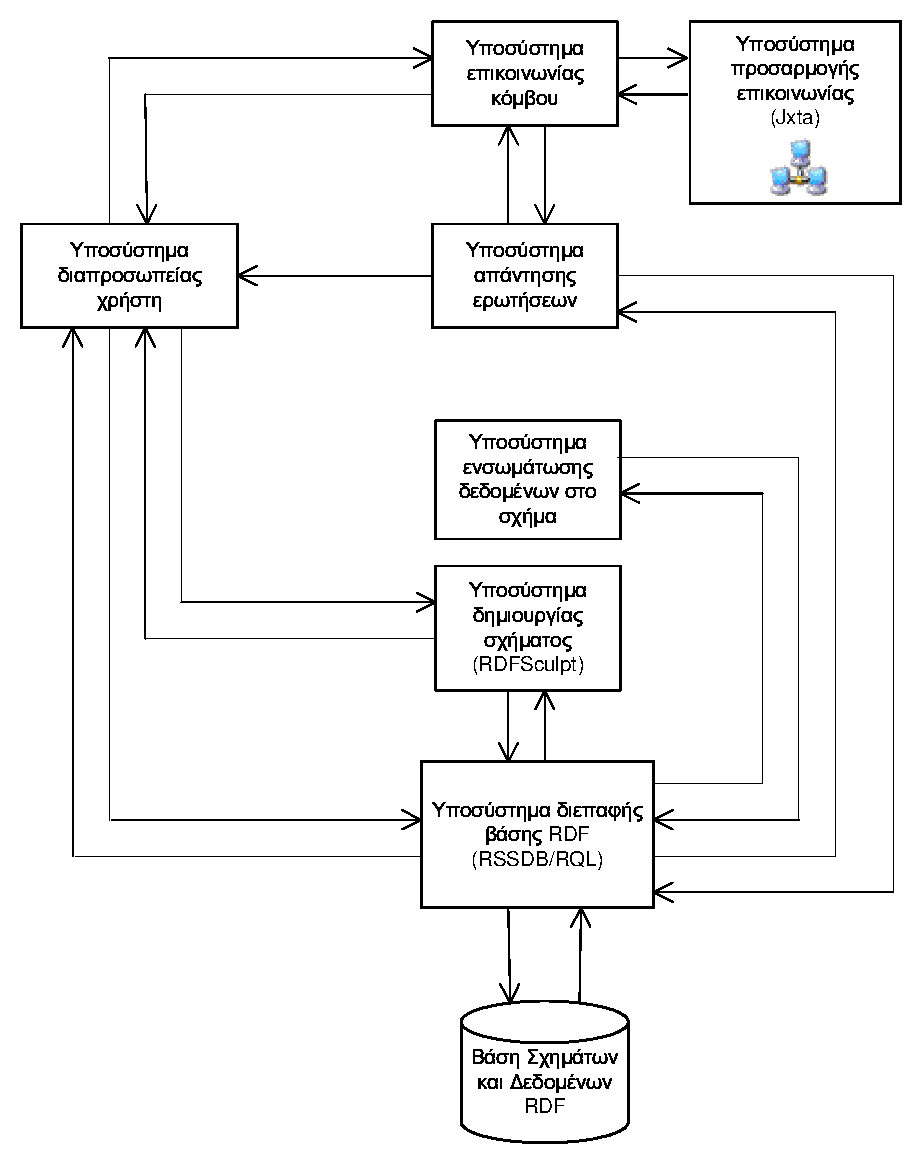
\includegraphics{static/figures/peerArchitecture.eps} \caption{Αρχιτεκτονική Απλού
Κόμβου}\label{figure4.1}
\end{figure}

Το Σχήμα~\ref{figure4.1} απεικονίζει .................


\subsection{Περιγραφή υποσυστημάτων}
Παρακάτω δίνεται λεπτομερής περιγραφή για καθένα από τα συστήματα
που αναφέραμε. Η περιγραφή αυτή γίνεται με βάση τα διαγράμματα
ροής δεδομένων.

\subsubsection{Υποσύστημα δημιουργίας σχήματος}
Το υποσύστημα αυτό ...............
	\chapter{\selectlanguage{greek}Υλοποίηση}
Στο κεφάλαιο αυτό περιγράφεται η υλοποίηση του συστήματος, με βάση
τη μελέτη που παρουσιάστηκε στο προηγούμενο κεφάλαιο. Αρχικά
παρουσιάζεται η πλατφόρμα και τα προγραμματιστικά εργαλεία που
χρησιμοποιήθηκαν. Στη συνέχεια δίνονται οι λεπτομέρειες υλοποίησης
για τους βασικούς αλγορίθμους του συστήματος καθώς και η δομή του
κώδικα.

\section{\selectlanguage{greek}Λεπτομέρειες υλοποίησης}
Στην ενότητα αυτή παρουσιάζονται οι βασικοί αλγόριθμοι που
αναπτύχθηκαν καθώς και λεπτομέρειες σχετικά με την υλοποίηση της
επικοινωνίας των κόμβων.

\subsection{Αλγόριθμοι}

\subsubsection{Αλγόριθμος εισαγωγής δεδομένων}
Όταν ένας κόμβος εισέρχεται για πρώτη φορά στο σύστημα, αρχικά
δημιουργεί το σχήμα που θέλει χρησιμοποιώντας το \en{RDFSculpt}.
Στη συνέχεια................

\noindent\texttt{Κατασκευή του διανύσματος \en{groupedMapping}. \\
Περιέχει ομαδοποιημένα τα} \texttt{στοιχεία} \texttt{του \en{mapping} που ανήκουν
στην ίδια κλάση. \\ Το διάνυσμα \en{groupedMapping} έχει τη μορφή: \\
$[[[[$Κλάση1,Κυριολεκτικό1$]$,Χαρακτηριστικό1$]$,$[[$Κλάση1,Κυριολεκτικό2$]$
\\,Χαρακτηριστικό2$]$,...$]$,$[[[$Κλάση2,Κυριολεκτικό3$]$,Χαρακτηριστικό3$]$,
$[[$Κλάση2,\\Κυριολεκτικό4$]$,Χαρακτηριστικό4$]$,...$]]$ }
\texttt{
\begin{tabbing}
Γι\=α κ\=άθε \=εγ\=γρ\=αφ\=ή \\
Δημιούργησε αντίγραφο του \en{groupedMapping}, που ονομάζεται \en{imapping} \\
Όσο το \en{imapping} έχει στοιχεία \\
\>Πάρε το πρώτο στοιχείο του διανύσματος έστω \en{classMapping} \\
\>\>Βάλε την κλάση που ανήκει στο πρώτο στοιχείο, στο διάνυσμα \\
\>\>\en{classesToWrite} \\
\>\>Όσο το διάνυσμα \en{classesToWrite} έχει στοιχεία \\
\>\>\>Πάρε το στοιχείο-κλάση που βρίσκεται στην αρχή του διανύσματος \\
\end{tabbing}
}

\noindent\textbf{Παράδειγμα} \\

Έστω ότι ο κόμβος έχει επιλέξει να συμμετέχει στο σύστημα με το \en{RDF} σχήμα που φαίνεται
στο Σχήμα.  Για τις ανάγκες του παραδείγματος θεωρούμε
ότι η όψη αυτή περιέχει μόνο μία εγγραφή.

...........................

\section{\selectlanguage{greek}Περιγραφή κλάσεων}
Στην ενότητα αυτή δίνεται μια σύντομη περιγραφή των κλάσεων,
των πεδίων και των μεθόδων που τις απαρτίζουν.

\subsection{\selectlanguage{greek}\en{public class FirstUi}}
\noindent Η κλάση αυτή κατασκευάζει την οθόνη εισαγωγής του χρήστη στο σύστημα.\\

\noindent\textbf{Πεδία}

\begin{itemize}
\item\src{private GridBagLayout blayout} \\
Το \en{layout} για όλα τα \en{Panel}.
\item\src{private GridBagConstraints con} \\
Τα \en{constraints} για το \en{layout}.
\item\src{private Icon arrowR} \\
Εικονίδιο για το κουμπί \en{Next}.
\end{itemize}

\noindent\textbf{Μέθοδοι}

\begin{itemize}
\item\src{public FirstUi()}\\
Ο κατασκευαστής της κλάσης ο οποίος καλεί την \en{createEntryFrame()}.
\item\src{private void createEntryFrame()}\\
Μέθοδος που κατασκευάζει το en{frame}.
\end{itemize}
	\chapter{Έλεγχος}
Στο κεφάλαιο αυτό γίνεται ο έλεγχος καλής λειτουργίας του
συτσήματος.

\section{Μεθοδολογία Ελέγχου}
Ο έλεγχος του συστήματος αυτού πραγματοποιήθηκε με τη χρήση ενός
σεναρίου λειτουργίας. Σύμφωνα με το σενάριο αυτό θεωρούμε ότι στο
σύστημα υπάρχουν τρεις κόμβοι (\en{peer1,peer2,peer3}). Θεωρούμε
επίσης ότι οι κόμβοι \en{peer2} και \en{peer3} έχουν ήδη σχήμα και
δεδομένα. 

Επίσης η τοπολογία του συστήματος έχει ως εξής: ο \en{peer2} είναι
γείτονας του \en{peer1} και ο \en{peer3} γείτονας του \en{peer2}.

Αρχικά λοιπόν θα δημιουργήσουμε σχήμα για τον κόμβο \en{peer1} και
στη συνέχεια θα εισάγουμε σε αυτό δεδομένα εξετάζοντας έτσι την
καλή λειτουργία του υποσυστήματος δημιουργίας σχήματος και του
υποσυστήματος εισαγωγής δεδομένων. Στη συνέχεια από τον κόμβο αυτό
στέλνουμε ερωτήσεις στους υπόλοιπους για τον έλεγχο του
υποσυστήματος απάντησης ερωτήσεων και επικοινωνίας κόμβων.

\section{Αναλυτική παρουσίαση ελέγχου}
Στην ενότητα αυτή παρουσιάζουμε αναλυτικά τον έλεγχο του
συστήματος σύμφωνα με το σενάριο που περιγράφηκε στην προηγούμενη
ενότητα.


	\chapter{Παράδειγμα Πίνακα}

\section{Συμπεράσματα}
Τα συστήματα ομότιμων κόμβων, προκειμένου να υποστηρίζουν πιο
εκφραστικές λειτουργίες αναπαράστασης και αναζήτησης δεδομένων,
εξελίχθηκαν στα συστήματα ομότιμων κόμβων τα οποία βασίζονται στις
τεχνολογίες του Σημασιολογικού Ιστού για την αναπαράσταση των
δεδομένων μέσω σχημάτων που τα περιγράφουν (\en{Schema-based
peer-to-peer systems}).

Συμπερασματικά το σύστημα που αναπτύχθηκε στα πλαίσια αυτής της
διπλωματικής είναι ένα πλήρες σύστημα ομότιμων κόμβων βασισμένο σε
σχήματα, το οποίο καθιστά δυνατή την αναζήτηση της πληροφορίας με
ένα διαφορετικό τρόπο απ' ότι τα προϋπάρχοντα  συστήματα.

\section{Μελλοντικές Επεκτάσεις}
Το σύστημα που αναπτύχθηκε στα πλαίσια αυτής της διπλωματικής
εργασίας θα μπορούσε να βελτιωθεί και να επεκταθεί περαιτέρω,
τουλάχιστον ως προς τρεις κατευθύνσεις. Συγκεκριμένα, αναφέρονται
τα ακόλουθα:

\begin{itemize}
\item Ενσωμάτωση διαδικασίας επιλογής σχήματος με βάση το οποίο ο
κόμβος θα συμμετέχει στο σύστημα. Έτσι όπως έχει σχεδιαστεί το
σύστημα, κάθε κόμβος έχει τη δυνατότητα να δημιουργήσει πολλά
σχήματα και να αποθηκεύσει δεδομένα σε περισσότερα από ένα. Ως
σχήμα του κόμβου (με βάση το οποίο απαντάει τις ερωτήσεις),
θεωρείται το τελευταίο στο οποίο αποθήκευσε δεδομένα. Η δυνατότητα
επιλογής θα του παρείχε περισσότερη ευελιξία.
\item Δυνατότητα αντιστοίχισης δεδομένων τα οποία να μην είναι
αποθηκευμένα σε βάση δεδομένων αλλά σε αρχεία. Η αποδέσμευση από
τη βάση δεδομένων θα έκανε το σύστημα πιο εύκολο στην εγκατάσταση
και τη χρήση.
\item Αξιολόγηση του συστήματος ως προς τη συμπεριφορά του αν
συμμετέχει σε αυτό μεγάλος αριθμός κόμβων \en{(scalability
testing)} και αν χρησιμοποιηθεί ένα πολύ μεγάλο καθολικό σχήμα. H
αξιολόγηση αυτή αφορά την ταχύτητα με την οποία ένας κόμβος
παίρνει απαντήσεις σε μια ερώτηση καθώς και την ποιότητα των
απαντήσεων.
\end{itemize}

%
	\begin{table}[!tb]
		\centering
		\caption{Πίνακας αλήθειας της λογικής συνάρτησης \en{F}}
		\small
		\renewcommand{\arraystretch}{1.3}
		\begin{tabular}{| c | c | c || c |}
			\hline               
		  	\textbf{\en{A}} & \textbf{\en{B}} &  \textbf{\en{C}} &   \textbf{\en{F}} \\
			\hline
				  0 & 0 & 0 & 0  \\
				  0 & 0 & 1 & 0  \\
				  0 & 1 & 0 & 1  \\
				  0 & 1 & 1 & 0  \\	
				  1 & 0 & 0 & 1  \\
				  1 & 0 & 1 & 0  \\
				  1 & 1 & 0 & 1  \\
				  1 & 1 & 1 & 0  \\
		  	\hline
		\end{tabular}
		\label{table07.01}
	\end{table}
%
	\chapter{Παράδειγμα Μαθηματικών Σχέσεων -- Εκφράσεων}

\section{Συμπεράσματα}
Τα συστήματα ομότιμων κόμβων, προκειμένου να υποστηρίζουν πιο
εκφραστικές λειτουργίες αναπαράστασης και αναζήτησης δεδομένων,
εξελίχθηκαν στα συστήματα ομότιμων κόμβων τα οποία βασίζονται στις
τεχνολογίες του Σημασιολογικού Ιστού για την αναπαράσταση των
δεδομένων μέσω σχημάτων που τα περιγράφουν (\en{Schema-based
peer-to-peer systems}).

Στα συστήματα αυτά κάθε \en{$\displaystyle y=\int_0^1f(x)dx$} \en{$y=\int_0^1f(x)dx$} κόμβος χρησιμοποιεί ένα σχήμα για την \en{$\displaystyle \sum_{i=0}^{100}a_i$}
αναπαράσταση των δεδομένων του. Όμως σε ένα σύστημα ομότιμων
κόμβων, κάθε κόμβος έχει διαφορετικές απαιτήσεις αναπαράστασης
δεδομένων. Επομένως πρέπει να υπάρχει ευελιξία στην επιλογή \en{$\displaystyle \frac{1}{1+x^2}$}
σχήματος. Τα συστήματα που έχουν προταθεί μέχρι τώρα και παρέχουν
αυτή την ευελιξία, για να είναι δυνατή η αναζήτηση πληροφορίας,
απαιτούν την ύπαρξη κανόνων αντιστοίχισης μεταξύ των σχημάτων με
βάση τους οποίους να μετασχηματίζονται οι ερωτήσεις. Όμως δεν
υποστηρίζεται ακόμα αυτόματη δημιουργία και δυναμική ανανέωση των
κανόνων, που είναι απαραίτητα για τα συστήματα ομότιμων κόμβων.
\begin{equation}
	y=\int_0^1f(x)dx
	\label{equation08.01}
\end{equation}

Η συνεισφορά της (\ref{equation08.01}) παρούσας διπλωματικής εργασίας έχει δύο σκέλη. Το
πρώτο αφορά τη δημιουργία ενός πλήρους συστήματος ομότιμων κόμβων
βασισμένο σε σχήματα \en{RDF} το οποίο παρέχει: (α) την υποδομή
για την επικοινωνία των κόμβων,(β) μηχανισμό δημιουργίας σχήματος,
(γ) μηχανισμό ενσωμάτωσης σχεσιακών δεδομένων στο σχήμα με τη
χρήση αντιστοιχίσεων που δημιουργεί ο χρήστης με τη βοήθεια
ειδικής διαπροσωπείας, (δ) ευέλικτη διαπροσωπεία χρήστη για τη
διατύπωση ερωτημάτων και (ε) μηχανισμό απάντησης και επεξεργασίας
ερωτήσεων.

Το δεύτερο σκέλος αφορά το γεγονός ότι το συγκεκριμένο σύστημα
προσφέρει μια σχετική ευελιξία ως προς την επιλογή του σχήματος
από τον κάθε κόμβο, ενώ ταυτόχρονα δίνει τη δυνατότητα
μετασχηματισμού ερωτήσεων χωρίς τη χρήση κανόνων αντιστοίχισης.
Συγκεκριμένα, τα σχήματα των κόμβων αποτελούν
υποσύνολα$-$όψεις$($\en{views}) ενός βασικού σχήματος που
ονομάζεται καθολικό σχήμα. Εκμεταλλευόμενοι λοιπόν το γεγονός ότι
τα σχήματα αυτά είναι συμβατά μεταξύ τους, έχουμε τη δυνατότητα
ελέγχου της ικανοποιησιμότητας μιας ερώτησης και μετατροπής της
όπου χρειάζεται, χρησιμοποιώντας τόσο το σχήμα του κόμβου όσο και
το καθολικό σχήμα.

Συμπερασματικά το σύστημα που αναπτύχθηκε στα πλαίσια αυτής της
διπλωματικής είναι ένα πλήρες σύστημα ομότιμων κόμβων βασισμένο σε
σχήματα, το οποίο καθιστά δυνατή την αναζήτηση της πληροφορίας με
ένα διαφορετικό τρόπο απ' ότι τα προϋπάρχοντα  συστήματα.

\section{Μελλοντικές Επεκτάσεις}
Το σύστημα που αναπτύχθηκε στα πλαίσια αυτής της διπλωματικής
εργασίας θα μπορούσε να βελτιωθεί και να επεκταθεί περαιτέρω,
τουλάχιστον ως προς τρεις κατευθύνσεις. Συγκεκριμένα, αναφέρονται
τα ακόλουθα:

\begin{itemize}
\item Ενσωμάτωση διαδικασίας επιλογής σχήματος με βάση το οποίο ο
κόμβος θα συμμετέχει στο σύστημα. Έτσι όπως έχει σχεδιαστεί το
σύστημα, κάθε κόμβος έχει τη δυνατότητα να δημιουργήσει πολλά
σχήματα και να αποθηκεύσει δεδομένα σε περισσότερα από ένα. Ως
σχήμα του κόμβου (με βάση το οποίο απαντάει τις ερωτήσεις),
θεωρείται το τελευταίο στο οποίο αποθήκευσε δεδομένα. Η δυνατότητα
επιλογής θα του παρείχε περισσότερη ευελιξία.
\item Δυνατότητα αντιστοίχισης δεδομένων τα οποία να μην είναι
αποθηκευμένα σε βάση δεδομένων αλλά σε αρχεία. Η αποδέσμευση από
τη βάση δεδομένων θα έκανε το σύστημα πιο εύκολο στην εγκατάσταση
και τη χρήση.
\item Αξιολόγηση του συστήματος ως προς τη συμπεριφορά του αν
συμμετέχει σε αυτό μεγάλος αριθμός κόμβων \en{(scalability
testing)} και αν χρησιμοποιηθεί ένα πολύ μεγάλο καθολικό σχήμα. H
αξιολόγηση αυτή αφορά την ταχύτητα με την οποία ένας κόμβος
παίρνει απαντήσεις σε μια ερώτηση καθώς και την ποιότητα των
απαντήσεων.
\end{itemize}
	\chapter{Επίλογος}

\section{Συμπεράσματα}
Τα συστήματα ομότιμων κόμβων, προκειμένου να υποστηρίζουν πιο
εκφραστικές λειτουργίες αναπαράστασης και αναζήτησης δεδομένων,
εξελίχθηκαν στα συστήματα ομότιμων κόμβων τα οποία βασίζονται στις
τεχνολογίες του Σημασιολογικού Ιστού για την αναπαράσταση των
δεδομένων μέσω σχημάτων που τα περιγράφουν (\en{Schema-based
peer-to-peer systems}).

Στα συστήματα αυτά κάθε κόμβος χρησιμοποιεί ένα σχήμα για την
αναπαράσταση των δεδομένων του. Όμως σε ένα σύστημα ομότιμων
κόμβων, κάθε κόμβος έχει διαφορετικές απαιτήσεις αναπαράστασης
δεδομένων. Επομένως πρέπει να υπάρχει ευελιξία στην επιλογή
σχήματος. Τα συστήματα που έχουν προταθεί μέχρι τώρα και παρέχουν
αυτή την ευελιξία, για να είναι δυνατή η αναζήτηση πληροφορίας,
απαιτούν την ύπαρξη κανόνων αντιστοίχισης μεταξύ των σχημάτων με
βάση τους οποίους να μετασχηματίζονται οι ερωτήσεις. Όμως δεν
υποστηρίζεται ακόμα αυτόματη δημιουργία και δυναμική ανανέωση των
κανόνων, που είναι απαραίτητα για τα συστήματα ομότιμων κόμβων.

Η συνεισφορά της παρούσας διπλωματικής εργασίας έχει δύο σκέλη. Το
πρώτο αφορά τη δημιουργία ενός πλήρους συστήματος ομότιμων κόμβων
βασισμένο σε σχήματα \en{RDF} το οποίο παρέχει: (α) την υποδομή
για την επικοινωνία των κόμβων,(β) μηχανισμό δημιουργίας σχήματος,
(γ) μηχανισμό ενσωμάτωσης σχεσιακών δεδομένων στο σχήμα με τη
χρήση αντιστοιχίσεων που δημιουργεί ο χρήστης με τη βοήθεια
ειδικής διαπροσωπείας, (δ) ευέλικτη διαπροσωπεία χρήστη για τη
διατύπωση ερωτημάτων και (ε) μηχανισμό απάντησης και επεξεργασίας
ερωτήσεων.

Το δεύτερο σκέλος αφορά το γεγονός ότι το συγκεκριμένο σύστημα
προσφέρει μια σχετική ευελιξία ως προς την επιλογή του σχήματος
από τον κάθε κόμβο, ενώ ταυτόχρονα δίνει τη δυνατότητα
μετασχηματισμού ερωτήσεων χωρίς τη χρήση κανόνων αντιστοίχισης.
Συγκεκριμένα, τα σχήματα των κόμβων αποτελούν
υποσύνολα$-$όψεις$($\en{views}) ενός βασικού σχήματος που
ονομάζεται καθολικό σχήμα. Εκμεταλλευόμενοι λοιπόν το γεγονός ότι
τα σχήματα αυτά είναι συμβατά μεταξύ τους, έχουμε τη δυνατότητα
ελέγχου της ικανοποιησιμότητας μιας ερώτησης και μετατροπής της
όπου χρειάζεται, χρησιμοποιώντας τόσο το σχήμα του κόμβου όσο και
το καθολικό σχήμα.

Συμπερασματικά το σύστημα που αναπτύχθηκε στα πλαίσια αυτής της
διπλωματικής είναι ένα πλήρες σύστημα ομότιμων κόμβων βασισμένο σε
σχήματα, το οποίο καθιστά δυνατή την αναζήτηση της πληροφορίας με
ένα διαφορετικό τρόπο απ' ότι τα προϋπάρχοντα  συστήματα.

\section{Μελλοντικές Επεκτάσεις}
Το σύστημα που αναπτύχθηκε στα πλαίσια αυτής της διπλωματικής
εργασίας θα μπορούσε να βελτιωθεί και να επεκταθεί περαιτέρω,
τουλάχιστον ως προς τρεις κατευθύνσεις. Συγκεκριμένα, αναφέρονται
τα ακόλουθα:

\begin{itemize}
\item Ενσωμάτωση διαδικασίας επιλογής σχήματος με βάση το οποίο ο
κόμβος θα συμμετέχει στο σύστημα. Έτσι όπως έχει σχεδιαστεί το
σύστημα, κάθε κόμβος έχει τη δυνατότητα να δημιουργήσει πολλά
σχήματα και να αποθηκεύσει δεδομένα σε περισσότερα από ένα. Ως
σχήμα του κόμβου (με βάση το οποίο απαντάει τις ερωτήσεις),
θεωρείται το τελευταίο στο οποίο αποθήκευσε δεδομένα. Η δυνατότητα
επιλογής θα του παρείχε περισσότερη ευελιξία.
\item Δυνατότητα αντιστοίχισης δεδομένων τα οποία να μην είναι
αποθηκευμένα σε βάση δεδομένων αλλά σε αρχεία. Η αποδέσμευση από
τη βάση δεδομένων θα έκανε το σύστημα πιο εύκολο στην εγκατάσταση
και τη χρήση.
\item Αξιολόγηση του συστήματος ως προς τη συμπεριφορά του αν
συμμετέχει σε αυτό μεγάλος αριθμός κόμβων \en{(scalability
testing)} και αν χρησιμοποιηθεί ένα πολύ μεγάλο καθολικό σχήμα. H
αξιολόγηση αυτή αφορά την ταχύτητα με την οποία ένας κόμβος
παίρνει απαντήσεις σε μια ερώτηση καθώς και την ποιότητα των
απαντήσεων.
\end{itemize}
% Παραρτήματα
	\appendix
	\chapter{Παράδειγμα Παραρτήματος}

\section{Πρώτη ενότητα}
Τα συστήματα ομότιμων κόμβων, προκειμένου να υποστηρίζουν πιο
εκφραστικές λειτουργίες αναπαράστασης και αναζήτησης δεδομένων,
εξελίχθηκαν στα συστήματα ομότιμων κόμβων τα οποία βασίζονται στις
τεχνολογίες του Σημασιολογικού Ιστού για την αναπαράσταση των
δεδομένων μέσω σχημάτων που τα περιγράφουν (\en{Schema-based
peer-to-peer systems}).

Συμπερασματικά το σύστημα που αναπτύχθηκε στα πλαίσια αυτής της
διπλωματικής είναι ένα πλήρες σύστημα ομότιμων κόμβων βασισμένο σε
σχήματα, το οποίο καθιστά δυνατή την αναζήτηση της πληροφορίας με
ένα διαφορετικό τρόπο απ' ότι τα προϋπάρχοντα  συστήματα.

\section{Μελλοντικές Επεκτάσεις}
Το σύστημα που αναπτύχθηκε στα πλαίσια αυτής της διπλωματικής
εργασίας θα μπορούσε να βελτιωθεί και να επεκταθεί περαιτέρω,
τουλάχιστον ως προς τρεις κατευθύνσεις. Συγκεκριμένα, αναφέρονται
τα ακόλουθα:

\begin{itemize}
\item Ενσωμάτωση διαδικασίας επιλογής σχήματος με βάση το οποίο ο
κόμβος θα συμμετέχει στο σύστημα. Έτσι όπως έχει σχεδιαστεί το
σύστημα, κάθε κόμβος έχει τη δυνατότητα να δημιουργήσει πολλά
σχήματα και να αποθηκεύσει δεδομένα σε περισσότερα από ένα. Ως
σχήμα του κόμβου (με βάση το οποίο απαντάει τις ερωτήσεις),
θεωρείται το τελευταίο στο οποίο αποθήκευσε δεδομένα. Η δυνατότητα
επιλογής θα του παρείχε περισσότερη ευελιξία.
\item Δυνατότητα αντιστοίχισης δεδομένων τα οποία να μην είναι
αποθηκευμένα σε βάση δεδομένων αλλά σε αρχεία. Η αποδέσμευση από
τη βάση δεδομένων θα έκανε το σύστημα πιο εύκολο στην εγκατάσταση
και τη χρήση.
\item Αξιολόγηση του συστήματος ως προς τη συμπεριφορά του αν
συμμετέχει σε αυτό μεγάλος αριθμός κόμβων \en{(scalability
testing)} και αν χρησιμοποιηθεί ένα πολύ μεγάλο καθολικό σχήμα. H
αξιολόγηση αυτή αφορά την ταχύτητα με την οποία ένας κόμβος
παίρνει απαντήσεις σε μια ερώτηση καθώς και την ποιότητα των
απαντήσεων.
\end{itemize}

%
	\begin{table}[!tb]
		\centering
		\caption{Πίνακας αλήθειας της λογικής συνάρτησης \en{F}}
		\small
		\renewcommand{\arraystretch}{1.3}
		\begin{tabular}{| c | c | c || c |}
			\hline               
		  	\textbf{\en{A}} & \textbf{\en{B}} &  \textbf{\en{C}} &   \textbf{\en{F}} \\
			\hline
				  0 & 0 & 0 & 0  \\
				  0 & 0 & 1 & 0  \\
				  0 & 1 & 0 & 1  \\
				  0 & 1 & 1 & 0  \\	
				  1 & 0 & 0 & 1  \\
				  1 & 0 & 1 & 0  \\
				  1 & 1 & 0 & 1  \\
				  1 & 1 & 1 & 0  \\
		  	\hline
		\end{tabular}
		\label{tableAppA.01}
	\end{table}
%
	\chapter{Απόδειξη της σχέσης (8.1)}
Στο κεφάλαιο αυτό παρουσιάζεται η μελέτη που έγινε για την
υλοποίηση του συστήματος. Αρχικά περιγράφεται η αρχιτεκτονική του
συστήματος και γίνεται ο διαχωρισμός του στα επιμέρους
υποσυστήματα, ενώ στη συνέχεια περιγράφονται οι εφαρμογές του
συστήματος.

\section{Ανάλυση - περιγραφή αρχιτεκτονικής}
Στην ενότητα αυτή παρουσιάζεται η ανάλυση του συστήματος και ο
χωρισμός του σε υποσυστήματα όσον αφορά την αρχιτεκτονική.

\subsection{Διαχωρισμός υποσυστημάτων}
Το σύστημα αποτελείται από τους απλούς κόμβους και ένα κόμβο
διαχειριστή. Στο σημείο αυτό αναλύουμε το σύστημα ενός απλού
κόμβου, το οποίο αποτελείται από τα εξής υποσυστήματα:

\begin{itemize}
\item Υποσύστημα δημιουργίας σχήματος.
\item Υποσύστημα ενσωμάτωσης δεδομένων στο σχήμα.
\item Υποσύστημα επικοινωνίας κόμβου.
\end{itemize}


\begin{figure}[!ht] \centering
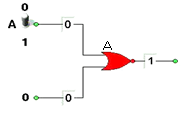
\includegraphics{static/figures/2.png} \caption{Προσομοίωση Πύλης \en{NOR}}\label{figureB.1}
\end{figure}

Το Σχήμα~\ref{figureB.1} απεικονίζει .................


\subsection{Περιγραφή υποσυστημάτων}
Παρακάτω δίνεται λεπτομερής περιγραφή για καθένα από τα συστήματα
που αναφέραμε. Η περιγραφή αυτή γίνεται με βάση τα διαγράμματα
ροής δεδομένων.

\subsubsection{Υποσύστημα δημιουργίας σχήματος}
Το υποσύστημα αυτό ...............	
	\cleardoublepage
% Βιβλιογραφία - Αναφορές
	\bibliography{back_matter/references}
% Συντομογραφίες - Αρκτικόλεξα - Ακρωνύμια
	\newcommand{\abbrevEN}[2]{\en{#1} \> \en{#2}\\ }
\newcommand{\abbrevGR}[2]{#1 \> #2\\ }

\chapter*{Συντομογραφίες - Αρκτικόλεξα - \\ - Ακρωνύμια}

\begin{tabbing}
%ta 'a' rythmizoun to platos ton dyo stilon
  aaaaaaaaaaaaaaaaa \= aaaaaaaaaaaaaaaaaaaaaa\kill
  \abbrevGR{βλπ}{βλέπε}
  \abbrevGR{κ.λπ.}{και λοιπά}
  \abbrevGR{κ.ο.κ}{και ούτω καθεξής}
  \abbrevGR{ΤΕΙ}{Τεχνολογικό Εκπαιδευτικό Ίδρυμα}
  \abbrevEN{BPF}{Band Pass Filter}
\end{tabbing}
% Γλωσσάριο
	\newcommand{\gloss}[2]{#1 \> \en{#2}\\ }

\chapter*{Απόδοση ξενόγλωσσων όρων}

\begin{tabbing}
%ta 'a' rythmizoun to platos ton dyo stilon
  aaaaaaaaaaaaaaaaaaaaaaaaaaaaaaaaaaa \= aaaa\kill
  \Large\textbf{Απόδοση} \> \Large\textbf{Ξενόγλωσσος όρος} \\
  \gloss{αδερφός}{sibling}
  \gloss{αμεταβλητότητα}{idempotency}
  %\gloss{αναγνωριστής}{identifier}
  \gloss{ανάκτηση πληροφορίας}{information retrieval}
  \gloss{αντιμεταθετικότητα}{commutativity}
  \gloss{απόγονος}{descedant}
  \gloss{απορρόφηση}{absorption}
  \gloss{βάση δεδομένων}{database}
  \gloss{γνώρισμα}{attribute}
  \gloss{διαπροσωπεία}{interface}
  \gloss{διαφορά}{difference}
  \gloss{δικτυακός κατάλογος}{portal catalog}
  \gloss{δικτυωτή δομή}{lattice}
  \gloss{δομικές επερωτήσεις}{structural queries}
  \gloss{δομικές σχέσεις}{structural relationships}
  \gloss{δομικό σχήμα}{schema}
  \gloss{εγκυρότητα}{validity}
  \gloss{ένωση}{union}
\end{tabbing}
%%%%%%%%%%%%%%%%%%%%%%%%%%%%%%%%%%%%%%%%%%%%%%%%%%%%
\backmatter
% Ευρετήριο Όρων
	\printindex
	\cleardoublepage

%%%%%%%%%%%%%%%%%%
%%%%%%%%%%%%%%%%%%

%% Δημιουργία ετικετών CD:

	\definecdlabeloffsets{0}{-0.65}{0}{0.55} % upper label x offset [cm] (default=0) /  upper label y offset [cm] (default=0) /  lower label x offset [cm] (default=0) /  lower  label y offset [cm] (default=0) -- For Q-Connect KF01579 labels use the following offset values: {0}{-0.65}{0}{0.55}

	\createcdlabel{Αναζήτηση και Εξόρυξη Πληροφορίας \\ σε Μεγάλες Βάσεις Αδόμητων Δεδομένων\\ με Μεθόδους Παράλληλης Επεξεργασίας}{Ολυμπία Ι. Τσάμου}{Μάιος}{2022}{8} % τίτλος πτυχιακής / όνομα συγγραφέα / μήνας / έτος / εύρος περιοχής τίτλου σε cm (προτεινόμενη τιμή: 8) 

%%
%% Δημιουργία εξωφύλλου θήκης CD:

	\createcdcover{Αναζήτηση και Εξόρυξη Πληροφορίας \\ σε Μεγάλες Βάσεις Αδόμητων Δεδομένων\\ με Μεθόδους Παράλληλης Επεξεργασίας}{Ολυμπία Ι. Τσάμου}{Μάιος}{2022}{10} % τίτλος πτυχιακής / όνομα συγγραφέα / μήνας / έτος / εύρος περιοχής τίτλου σε cm (προτεινόμενη τιμή: 10) 

%%
	\pagebreak
	\thispagestyle{empty}
\end{document}